\documentclass[12pt]{article}
\usepackage{graphicx}
\usepackage{hyperref}


\title{Document}
\author{Jesús y Dani}

\begin{document}


\section{Esto es un título}
\subsection{Esto es un subtítulo}
\subsubsection{Esto es un subsubtítulo}

Aquí comienza un texto que puede contener palabras en \textbf{negrita}, en \textit{cursiva} y \underline{subrayadas}. 
Puede contener también \href{https://ejemplo.com"}{enlaces}.
Además, se pueden empezar párrafos como el siguiente:

Esto es un párrafo de un documento HTML que termina con un salto de línea.\\

Se pueden ver también imágenes como la siguiente:\\


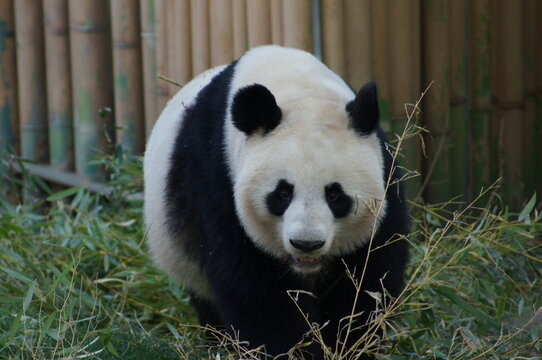
\includegraphics[width=300px, height=200px]{image.png}

Además se incluye una lista no ordenada:
\begin{itemize}
	\item Esto
	\item Es una lista
	\item No ordenada
\end{itemize}


Y una lista ordenada
\begin{enumerate}
	\item Esto
	\item Es una lista
	\item Ordenada
\end{enumerate}


Se añade también una tabla con 3 columnas y cabecera

\begin{tabular}{|c|c|c|}
	\hline
	\textbf{Esto} & \textbf{Es la} & \textbf{Cabecera} \\
	\hline
	Esto & Es el resto & de la tabla \\
	\hline
\end{tabular}


Se añade también una tabla con 2 columnas y sin cabecera 

\begin{tabular}{|c|c|}
	\hline
	Esto es & otra tabla \\
	\hline
	Esto & Es el resto \\
	\hline
\end{tabular}



\end{document}


